\chapter{Contexte : Colonie d'abeilles, Biologie et Complexité}
\label{ChapitreContexte}
	
	Les insectes sociaux sont depuis longtemps étudiés pour leur capacité à se répartir dynamiquement le travail, sans l'aide d'un contrôle central. Ce chapitre présente tout d'abord les principales notions de complexité et détaille ensuite plusieurs exemples de phénomènes complexes que l'on peut retrouver dans la vie d'une colonie d'abeilles. Nous verrons dans le chapitre suivant quelques modèles Multi-Agents présents dans la littérature servant à modéliser ces systèmes.

	
		\section{Systèmes Complexes}
		
			Il n'existe à ce jour pas de définition précise de ce qu'est un système complexe \cite{heylighen_complexity_2008}, du fait de l'étendue des domaines et cas d'applications concernés. En général, un système complexe peut être vu comme composé d'une multitude de composants (ou sous-systèmes) hétérogènes ne communiquant que très peu entre eux, formant un tout par leurs nombreuses interactions mutuelles. Un système complexe est un bon exemple de l'adage "Le tout vaut plus que la somme des parties" qui serait d'Aristote \cite{edmonds_what_1995}. Les notions de chaos, d'interactions locales et d'imprévisibilité sont souvent citées dans la littérature. Un système complexe ne peut pas être anticipé par le calcul, le seul moyen d'en connaitre l'état futur est de l'observer. 
			Ceci est notamment lié à ses propriétés \textit{émergentes}. Dans la littérature, une propriété est dite émergente lorsqu'elle possède trois caractéristiques \cite{breckling_emergent_2005} :
			\begin{enumerate}
				\item une propriété qui n'existe pas au niveau des sous-systèmes isolés;
				\item une propriété de haut niveau engendrée par les interactions entre sous-systèmes;
				\item une propriété qui apparait à un niveau du système n'est pas déductible uniquement en observant les propriétés des sous-systèmes.
			\end{enumerate}
			
			\subsection{Émergence et Auto-Organisation}
			
			Nous parlons ainsi d'émergence lorsque des comportements apparaissent grâce à des interactions entre différents composants, et que ces comportements sont absents lorsque ces mêmes composants sont étudiés séparément. Les propriétés émergentes sont le plus souvent imprévisibles du point de vue de chaque sous-système, donnant ainsi cette propriété aux systèmes complexes. Toutes ces émergences de comportements génèrent un système qui peut être dit chaotique. 
			Suivant les théories du chaos, ou "l'effet papillon", ces systèmes sont alors hautement imprévisibles et de légères variations de paramétrage ou de conditions initiales peuvent avoir de grandes conséquences sur le comportement global du système : "petit changement, grandes conséquences".
			
			Un système fait preuve d'\textit{auto-organisation} dès que "l'arrangement de ses sous-systèmes est non-aléatoire" \cite{goos_self-organisation_2003}. Plus généralement, un système fait preuve d'auto-organisation lorsqu'il démontre des capacités d'organisation sans contrôle explicite extérieur, mais à la suite de contraintes et/ou mécanismes internes engendrées par des interactions entre ses composants. Nous obtenons donc un système dynamique, capable de maintenir une forme stable et des états transitoires. Il n'est pas rare d'observer parmi ces mécanismes d'organisation des propriétés émergentes. Nous pouvons alors parler d'auto-organisation émergente, mais il est important de différencier ces deux termes : l'auto-organisation n'est pas systématiquement émergente, et des propriétés émergentes peuvent ne pas participer à l'auto-organisation d'un système, elles peuvent même l'empêcher.
			
			\begin{figure}
			\centering
			\begin{subfigure}{0.45\textwidth}
        		\centering
         		\includegraphics[height=.2\textheight]{Pictures/Figures/RetroActionBomb.png}
         		\caption{}
         		\label{bomb}
     		\end{subfigure}
     		\hfill
			\begin{subfigure}{0.45\textwidth}
        		\centering
         		\includegraphics[height=.2\textheight]{Pictures/Figures/RetroActionSun.png}
         		\caption{}
         		\label{sun}
     		\end{subfigure}
			\caption{Boucles de rétroactions simplifiées du fonctionnement d'une bombe nucléaire à fission, ou bombe A (a) et de l'équilibre hydrostatique du soleil (b).}{Un lien bleu se terminant par une flèche indique un renforcement, par exemple, la Pression au centre du Soleil vient augmenter son Rayon. Un lien rouge se terminant par un cercle indique une réduction : la Gravité à tendance à réduire le Rayon du soleil, en appliquant une force constante de toute part.}
			\label{RetroActions}
			\end{figure}
			
			\subsection{Boucles de Rétro-Action}
		
		Clés dans cette organisation, les interactions multiples entre les différentes composantes du système font le plus souvent apparaitre des boucles de rétroactions. Une boucle de rétroaction est un processus qui lie un effet à sa propre cause. En électronique, cela consiste à brancher la sortie d'un composant à l'une de ses entrées. Les boucles de rétroaction se présentent sous deux formes, les rétroactions positives et négatives. Les boucles de rétroactions positives consistent en des phénomènes de renforcement, d'accélération. Nous parlons alors dans le langage courant de "cercle vicieux ou vertueux". Une bombe nucléaire à fission fonctionne avec ce principe, une fission va en déclencher plusieurs autres, qui vont elles-mêmes en déclencher bien d'autres, sous une forme d'emballement exponentiel. La Figure \ref{bomb} illustre cet exemple, montrant l'amplification constante de la réaction, où chaque fission va augmenter le nombre de fissions réalisées par la bombe, par le biais d'émission de neutrons. Sans autre mécanisme pour les réguler, ce sont des phénomènes très transitoires. Les autoroutes de fourmis, de leur côté, utilisent un mécanisme de renforcement pour marquer les pistes avec des phéromones. Les fourmis viennent déposer des phéromones sur leur route lorsqu'elles reviennent d'une source avec de la nourriture. Ces phéromones attirent de nouvelles fourmis, qui vont alors remonter la piste et participer a la collecte de ressource. A leur retour, elles vont aussi déposer des phéromones, amplifiant rapidement l'attraction de ce chemin, le transformant rapidement en ce qui est surnommé une "autoroute". Ces phéromones s'évaporent, mais pour l'instant cette évaporation est largement compensée par les nouveaux dépôts de phéromones sur le chemin. En revanche, lorsque la source est épuisée, les phéromones ne sont plus renouvelées, l'évaporation n'est plus contre balancée, l'attraction du chemin diminue jusqu'à ne plus attirer aucune fourmis.
		Les boucles de rétroaction négatives consistent en mécanismes régulateurs, stabilisant un système vers un équilibre. Nous pouvons en trouver de toutes sortes, sous bien des formes. Le soleil par exemple, voit sa forme maintenue, par une boucle de rétroaction négative, à ce qui est appelé un équilibre hydrostatique \cite{haubold_analytic_1992} : lorsque son cœur réalise la fusion nucléaire, il crée une importante force en son centre, le faisant s'étendre. Le soleil gonfle alors et fait ainsi baisser la pression en son centre, le nombre de fusions est alors légèrement réduit. La force poussant le soleil à s'étendre est alors contrée par la gravité, le poussant de toute part vers son centre. Mais du même temps, la pression en son centre remonte, les fusions reprennent de plus belle et il gonfle à nouveau : le soleil danse légèrement autour de son point d'équilibre. La Figure \ref{sun} illustre ces interactions, et montre la rétroaction entre la pression et le rayon du soleil : augmenter la pression augmente le rayon du soleil, noté par une flèche bleue. Or, augmenter le rayon réduit la pression, noté par un lien rouge se terminant par un cercle.
		
		Ainsi, une boucle de rétroaction peut être une propriété émergente d'un système complexe, et joue un rôle dans son auto-organisation.
			
			Pour récapituler, un système complexe est composé d'une multitude de composants hétérogènes interagissant mutuellement avec des communications limitées. Ils sont imprévisibles et voient la plupart de leurs propriétés émerger des interactions entre composants, sous la forme de boucles de rétroactions.
			
			Un bel exemple de tels systèmes auxquels nous sommes soumis tous les jours est le climat. De faibles interactions qui peuvent paraitre insignifiantes ont de grandes répercussions sur le système dans son ensemble. Nous augmentons d'un demi degré la température des océans et ce sont les courants marins, les vents et tempêtes, les chaines alimentaires et bien d'autres qui se dérèglent. Augmenter de quelques points le pourcentage de gaz à effet de serre dans l'atmosphère et le circuit s'emballe et réchauffe le tout, augmentant la fréquence d'événements violents etc \cite{allen_2018_2018}. Une grande quantité d'entités, jusqu'à l'échelle moléculaire, vont interagir entre elles, faisant varier leur température, leur pression, leur absorption et réflexion de la lumière, altérant par la même occasion le climat sur une échelle planétaire, affectant jusqu'à notre mode de vie. Le climat est en bonne partie imprévisible, des modèles de plus en plus complexes sont mis en places et constamment améliorés par les météorologues afin d'affiner leurs prévisions.
						
			Nous allons maintenant constater en quoi une colonie d'abeilles\footnote{La ruche désigne l'objet, souvent une boite pour les abeilles domestiques, où les abeilles vivent. La colonie désigne l'ensemble des abeilles vivant en société, dans la ruche.} est un bon représentant de la grande famille des systèmes complexes : aucun contrôle central et des dizaines de milliers d'individus hétérogènes dotés de moyens de communication limités interagissant massivement entre eux, créant des boucles de rétroactions comportementales, chimiques mais aussi physiologiques.
			
			

	
		\section{Abeilles et Systèmes complexes}	
		\label{sectionBio}	
			Une colonie classique d'abeilles domestiques \textit{Apis Melifera} héberge en moyenne quelques dizaines de milliers d'individus, 50 000 est un nombre qui revient souvent. Tous ces individus ont des besoins en nourritures et en eau, mais le couvain, regroupant tous les stades de vie de l'abeille avant sa phase adulte, demande un tout autre niveau d'attention : nourriture spéciale, température précise, cellules de cires propres etc. Tous ces besoins créent une chaine logistique impressionnante, que des apiculteurs observent depuis des milliers d'années \cite{oldroyd_domestication_2012}. En effet, les abeilles (et bien d'autres insectes sociaux) arrivent à survivre et même à s'épanouir sans aucun contrôle central, aucun individus spéciaux chargés du management ou de la surveillance des stocks. Au fil de sa vie, une abeille va endosser différents rôles au sein de cette chaine, que nous allons décrire \cite{winston_biology_1991, winston_role_1991, seeley_age_1991}. 
			
			Emblématique de la colonie d'abeilles et présentant des différences physiques notables, la reine, plus grande que les autres abeilles, est chargée de pondre près d'un œuf par minute en moyenne sur toute sa vie. Elle est en permanence entourée d'une "cour royale", des abeilles adultes qui viennent la lécher de tous côtés, attirées par ses phéromones puissantes. Elles vont ensuite répandre les phéromones royales dans toute la ruche, permettant ainsi à l'ensemble de la colonie de sentir la présence de la reine. Souvent ces abeilles sont des nourrices, elles sont chargées de nourrir le couvain. Elles parcourent la ruche à la recherche de miel et de pollen afin de concocter un liquide calorifique dont les larves se nourrissent. Parfois, une recette alternative encore plus riche, la gelée royale, est donnée à des larves spécialement sélectionnées pour devenir de nouvelles reines.
			
			\begin{figure}
			\centering
			\includegraphics[width=0.45\textwidth]{Pictures/Figures/larvaLeft.jpg}
			\includegraphics[width=0.45\textwidth]{Pictures/Figures/larvaRight.jpg}
			\caption[Tirée de Winston, 1991 \cite{winston_biology_1991}. Croissance de l'oeuf à l'émergence, pour les ouvrières, les mâles et les reines.]{Tiré de Winston, 1991 \cite{winston_biology_1991}. Croissance de l'oeuf à l'émergence, pour les ouvrières, les mâles et les reines. La croissance se passe en trois étapes, oeuf, larve, nymphe, dont les durées varient selon l'abeille. Pour les ouvrières ces étapes sont en moyenne de 3 jours en tant qu'œuf, puis de 6 jours en tant que larve et enfin de 12 jours en tant que nymphe.}
			\label{LarvaDev}
			\end{figure}
			
			Les larves ne sont que des systèmes digestifs autonomes. Elles ingurgitent de grandes quantités de nourriture par rapport à leur poids, pour assurer leur croissance rapide, et leur permettre de devenir adultes. La reine pond des œufs, qu'elle dépose au fond de cellules. Ces cellules doivent être bâties par des ouvrières cirières, et nettoyées avant que la reine ne puisse y pondre. Une fois pondu, un œuf d'ouvrière va mettre trois jours pour évoluer en larve, puis consommer son mélange de miel et de pollen pendant six jours, avant de devenir une nymphe, étape importante où la larve va se métamorphoser progressivement en sa forme finale, une abeille adulte, 21 jours après la ponte. La Figure \ref{LarvaDev} tirée des travaux de Winston \cite{winston_biology_1991} illustre les temps de croissances des différents types d'abeilles, de l'œuf à l'émergence, passant par la larve et la nymphe. En effet, les reines, les ouvrières et les mâles ne partagent pas les même temps de croissance, une reine émerge 16 jours après que son œuf ait été pondu, alors que cette durée est de 24 jours pour les mâles. Dès qu'une larve passe au stade de nymphe, elle est repérée par une ouvrière cirière qui va méthodiquement operculer la cellule : créer une sorte de toit afin d'enfermer la nymphe qui devra ouvrir sa cellule elle même, dans ses premières heures d'adulte, à l'aide de ses nouvelles mandibules.
			
			Pour que toute cette croissance se passe bien, la température du couvain doit être exactement de 35°C. Un écart de l'ordre du degré peut engendrer des pertes colossales, et mettre la colonie en péril. Certaines abeilles effectuent alors des tâches de thermo-régulation, lorsqu'il fait trop chaud ou trop froid, afin de toujours garder une température optimale dans la ruche.

			
			Les abeilles à miel sont surtout célèbres pour leur butinage, rôle tenu par les "butineuses". Celles-ci sélectionnent les meilleurs sites de ressources sur une surface de plus de 300km² \cite{riviere_modemulti-agent_2021} et ramènent nectar, pollen et eau à la colonie. Certaines abeilles vont spontanément quitter la ruche sans destination, dans le seul but de trouver une nouvelle source de nectar. Ces butineuses sont appelées des "scouts", ou des "éclaireurs". Elles repèrent les fleurs grâce à leurs yeux à facettes sensibles aux ultra-violets, que les fleurs ont appris à bien réfléchir dans une co-évolution avec les pollinisateurs \cite{thompson_concepts_1989}. Une fois rentrée, la butineuse cherche une "receveuse" : elle lui donne une partie de sa charge de nectar. Les butineuses donnent ainsi leur récolte à trois ou quatre receveuses. Ensuite, elles viennent déposer leurs ballots de pollen dans des cellules proches du couvain, puis repartent butiner ou vont se reposer. 
			
			Dans le même temps, les receveuses vont déposer le nectar reçu dans des cellules, toujours très hautes sur le cadre. Certaines iront aussi tasser les ballots de pollen dans leurs cellules, afin de ne pas perdre de place. Le nectar est alors prêt à subir ses transformations pour devenir du miel. Certaines abeilles vont alors venir "cracher" sur le nectar, afin d'y déposer leurs enzymes qui feront le travail de transformation. Elles y déposent du même coup une substance antiseptique, s'assurant ainsi que le miel ne sera pas contaminé par de mauvaises bactéries ou virus (c'est en partie ce qui lui confère ses propriétés médicales). Ensuite, pendant ce travail d'enzymes, des "ventileuses" viendront se placer au dessus du miel et battre frénétiquement des ailes. Elles ajustent ainsi l'hygrométrie du miel, l'amenant très précisément à 15\% d'humidité, parfait pour la conservation.
			
			Toutes ces ouvrières sont sœurs ou demi-sœurs. Elles ont la plupart du temps toutes la même mère, mais pas forcément le même père. Au moment de la ponte, la reine "choisi" de féconder ou non son œuf. Les cellules où sont pondus les œufs de mâles sont plus grandes que celles des femelles, l'hypothèse la plus répandue est que les cellules plus petites des femelles viennent comprimer l'abdomen de la reine, provoquant ainsi la fécondation de l'œuf ainsi déposé, sans réelle décision au moment de la ponte. Un œuf fécondé donnera une femelle, un œuf non fécondé donnera un mâle d'après un mécanisme appelé "Parthénogenèse". 
			Les mâles ont une vie très particulière : ils sont incapables de quoi que ce soit, ni de se laver, ni de se nourrir seuls, et ne font rien dans la colonie. Dès que la situation se gâte et que les ressources se font rares (souvent au début de l'hiver), ce sont les premiers à être chassés de la colonie. Lors des vols nuptiaux, ils s'envolent vers un point de rencontre défini, localisent une reine et la fécondent. Ces points de rencontres regroupent les mâles et reines de nombreuses colonies des environs. Ils meurent instantanément après l'acte. Une reine est ainsi fécondée par une douzaine de mâles et va garder leur semence dans sa spermathèque et s'en servir tout au long de sa vie.
			
			Nous allons désormais nous intéresser plus en détails à ces nombreux mécanismes de contrôle et à l'auto-organisation de la répartition des tâches qu'ils induisent au sein de la colonie.
			
		\section{Auto-Organisation de la Colonie}
			Afin d'assurer le bon fonctionnement et l'épanouissement de la colonie, chaque individu la composant doit effectuer un certain nombre de tâches lorsqu'elles sont nécessaires, et sans aucun contrôle central. Par exemple, la colonie ne compte pas d'individus dont la seule tâche est de surveiller la température et, au besoin, d'assigner une équipe à sa régulation pendant un certain temps. Chaque individu utilise ses perceptions locales, internes et/ou externes, pour savoir quel travail réaliser, ainsi nous parlons de l'auto-organisation de l'allocation du travail. Nous nous intéressons ici en particulier aux phénomènes complexes suivants et à leurs mécanismes d'auto-organisation (dont leurs boucles de rétroaction) :
			
			
			\begin{itemize}
				\item la thermorégulation : la température est maintenue précisément à 35°C au niveau du couvain;
				\item la sélection des meilleures sources de nourritures par les butineuses par le biais de leur mécanisme de recrutement;
				\item la régulation de l'âge du premier butinage en fonction des demandes du couvain.
			\end{itemize}

			\subsection{Thermorégulation}	
			
			Lorsqu'il fait légèrement trop chaud dans la ruche, nous trouvons des abeilles thermo-régulatrices : elles battent des ailes sur le couvain et/ou au niveau de la sortie de la ruche pour créer un courant d'air et rafraichir la ruche. Certaines vaporisent même de l'eau dans la ruche pour aider à faire chuter la température. Lorsqu'il fait froid, les abeilles se resserrent progressivement au dessus du couvain, afin de créer ce qui est appelé la "grappe" et tenir le couvain au chaud grâce à leurs corps. Si leur simple présence ne suffit plus, elles peuvent actionner certains de leurs muscles afin de générer un peu plus de chaleur, ce qui arrive pendant l'hiver, phase critique pour la colonie. Si la grappe est trop petite pour recouvrir l'ensemble de couvain alors une bonne partie de ce dernier, en périphérie, n'aura pas été protégé par les adultes et va mourir, on l'appelle alors le "couvain refroidi".
					
			Un des points clés de cette capacité est que chaque individu a des "tolérances" légèrement différentes. Une diversité qui provient notamment de la présence des "demi-sœurs", dont nous avons parlé ci-dessus. J. Jones et.al. \cite{jones_honey_2004} ont montré que la capacité des abeilles à réguler précisément la température est liée à cette diversité génétique. En effet, pour que la colonie régule correctement, il est important d'éviter que trop d'individus ne réchauffent ou ne refroidissent la ruche ne même temps, afin de ne pas osciller entre trop chaud et trop froid. La diversité génétique modifie légèrement les seuils de tolérances des abeilles, qui vont alors progressivement réguler la température. Lorsqu'elle sera légèrement trop haute, seules certaines abeilles ventileront, les autres, de part leur tolérance plus élevée, ne vont pas participer. Ainsi, si l'action des premières est suffisante, la température revient doucement au bon niveau. Si la température continue de monter, alors de plus en plus d'abeilles la verront atteindre leur seuil de tolérance, et se joindront à l'effort.
			
			De cette manière, chaque individu mesure et juge localement la température actuelle autour de lui, et prend alors la décision de réchauffer, refroidir, ou réaliser d'autres devoirs. Sa position dans la ruche et sa sensibilité personnelle vont entrer en compte dans cette décision. Ainsi, par l'action autonome de chacun des individus, la température du couvain ne s'écarte jamais plus d'un degré de 35°C. La colonie a toujours un nombre optimal d'individus régulant la température, permettant de répondre parfaitement au besoin sans délaisser les autres tâches.
			
			\subsection{Sélection des meilleures sources de nectar}
			
			\begin{figure}
			\centering
			\includegraphics[width=0.8\textwidth]{Pictures/Figures/Waggle.JPG}
				\caption{Tiré des travaux de T.D. Seeley \cite{seeley_wisdom_1995} sur la Waggle Dance.}{ L'abeille effectuant la Waggle Dance indique non seulemement la distance de la source à la ruche, mais aussi sa direction, en prenant le soleil comme référence. Danser vers le haut, avec un angle de 0°, indique ainsi d'aller directement vers le soleil.}
			\label{Waggle}
			\end{figure}
			
			
	\begin{figure}
	\centering
	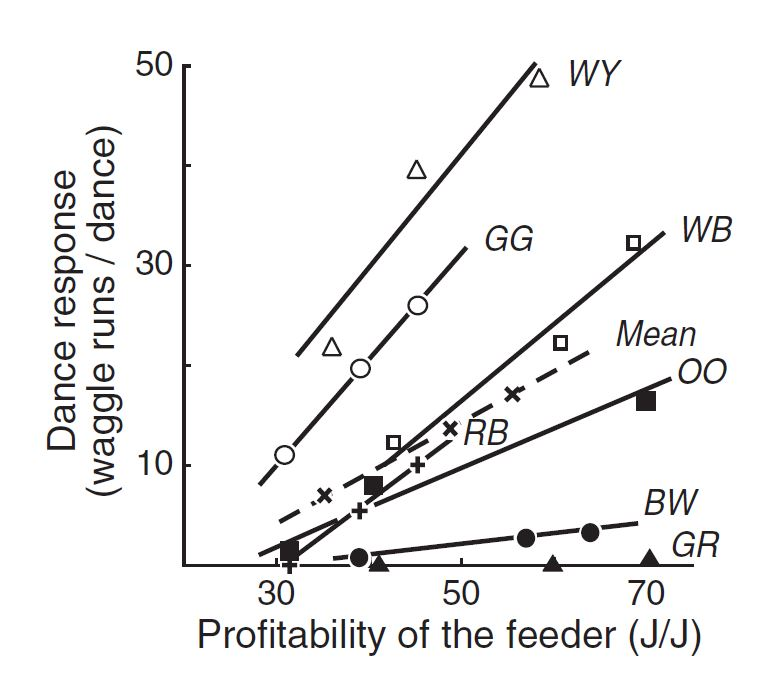
\includegraphics[width=0.45\textwidth]{Pictures/Graphs/SeeleyWaggles.JPG}
	\caption[Tiré des travaux de T.D. Seeley \cite{seeley_wisdom_1995}. En abscisses la profitabilité de la source, et en ordonnées le nombre de 8 (de \textit{Waggle}) réalisés par chaque abeilles par danse après être rentrée à la ruche.]{Tiré des travaux de T.D. Seeley \cite{seeley_wisdom_1995}. En abscisses la profitabilité de la source, et en ordonnées le nombre de danses répétées par chaque abeille après être rentrée à la ruche. 7 butineuses ont été observées après avoir récolté du nectar sur une source contrôlée, leurs danses ont été enregistrées. Ils ont ensuite montré que le nombre de \textit{Waggle} et leurs durées sont directement liés à la profitabilité de la source.}
	\label{SeeleyWaggles}
	\end{figure}
			
			\begin{figure}
			\centering
			\includegraphics[width=0.8\textwidth]{Pictures/Graphs/SeeleyNSRemix.JPG}
				\caption[Résultats redessinés d'une expérience de T.D. Seeley \cite{seeley_collective_1991} montrant les capacités des butineuses à sélectionner les meilleurs sources.]{Résultats redessinés d'une expérience de T.D. Seeley \cite{seeley_collective_1991} montrant les capacités des butineuses à sélectionner les meilleurs sources. La source Sud commence à 2.5mol/L de sucre, et la source Nord à 1.0mol/L. La source Sud est donc la plus profitable. À midi, la source Sud passe à 0.75mol/L et la source Nord est augmentée à 2.5mol/L. La source Nord devient alors la plus profitable. Cette cassure est visible sur les courbes, où la source Sud, alors bien exploitée, se voit abandonnée en masse, tandis que l’affluence à la source Nord augmente subitement, montrant l’auto-organisation rapide des butineuses.}
			\label{SeeleyNS}
			\end{figure}
	
			
			
			Lors de la collecte du nectar, les butineuses sont très sélectives et préfèrent les nectars aux hautes teneurs en sucres sur des fleurs situées le plus proche possible de la ruche. La colonie utilise donc un système de recrutement afin d'allouer ses effectifs de butineuses de manière optimale et dynamique, préférant les sources proches et nutritives \cite{riviere_modemulti-agent_2021}.
	
	Avant de décoller, l'abeille recruteuse va se mettre à danser la \textit{"Waggle Dance"}, en forme de 8. La Figure \ref{Waggle}, tirée des travaux de T.D. Seeley \cite{seeley_wisdom_1995}, illustre rapidement le fonctionnement de cette danse, réalisée sur une zone bien définie de la ruche, proche de l'entrée, appelée la "piste de danse". La \textit{Waggle Dance} a un objectif double. Le premier consiste à communiquer la position de la source de nectar, en indiquant sa direction par rapport au soleil ainsi que sa distance à la ruche, pour permettre aux autres de la retrouver. Le second est plus indirect : plus la source est sucrée et proche, et donc profitable, plus l'abeille va danser longtemps, et même répéter la danse dans plusieurs endroits de la ruche. Une danse plus longue offre plus de temps à d'autres abeilles de venir la suivre et apprendre la position de cette nouvelle source. Ainsi, plus la source est profitable, plus la recruteuse va communiquer la position à de nombreuses butineuses. La Figure \ref{SeeleyWaggles} est tirée des travaux de T.D. Seeley \cite{seeley_wisdom_1995} et illustre empiriquement que les abeilles dansent de manière plus intense pour des sources plus sucrées.
			
			Une fois recrutées, les nouvelles butineuses se rendent à la source et répètent le processus : collecter, juger, rentrer et parfois recruter. Là encore, la diversité est clé : différents profils génétiques poussent certaines abeilles à danser pour des sources moins profitables, d'autres à très peu danser (maximisant ainsi le butinage), et même certaines à tout simplement abandonner la source. Nous pouvons voir sur la Figure \ref{SeeleyWaggles} que les abeilles labellisées "GR" et "BW" sont plus sélectives, là où les abeilles "WY" et "GG" le sont moins. Communiquer des sources de faible qualité va permettre à la colonie d'y maintenir un faible contingent. Ce contingent alors moins utile dans l'immédiat sert de surveillance, car les teneurs en sucres des nectars de différentes fleurs peuvent fortement varier selon les saisons mais aussi pendant la journée. 
			Une source de faible qualité peut devenir une source extrêmement intéressante en quelques heures. Le groupe alors déjà présent peut observer ce changement et déjà danser, pour avertir les autres, gagnant ainsi un temps précieux de re-découverte de la source mais aussi le temps d'amorcer une réponse conséquente. Gagner du temps sur une réaction exponentielle est toujours extrêmement précieux. 
			C'est en effet une boucle de rétroaction positive, plus il y a d'abeilles à apprécier la source plus il y aura de recruteuses, augmentant ainsi encore le nombre de recruteuses par la suite.
			
			 T.D. Seeley et son équipe ont réalisé une expérience mettant en valeur cette aptitude, en plaçant deux sources de nectar aux teneurs en sucre contrôlables aux alentours d'une ruche \cite{seeley_collective_1991}. Ils ont pu obtenir un grand nombre d'information en observant à la fois le comportement des abeilles dans la ruche, mais aussi sur chaque source artificielle. Une source, au nord de la ruche, était remplie avec un nectar à 1.0 mol/L de sucre, et l'autre au sud était quant à elle remplie d'un nectar sucré à 2.5 mol/L. 
			La source sud est alors largement privilégiée par les butineuses, tandis qu'une faible population de butineuses exploite la source nord. À midi, la source sud est abaissée à 0.75 mol/L de sucre, et la source nord est montée à 2.5 mol/L. Alors, la source sud est abandonnée en quelques heures au profit de la source nord. La Figure \ref{SeeleyNS} illustre les résultats de cette expérience, où les auteurs ont observé le nombre de butineuses sur chaque source pendant la journée. Ils ont ainsi mis en valeur l'adaptation de la colonie à un changement rapide d'environnement dans un temps relativement court, ses effectifs ont bien été redirigés vers la source la plus profitable.
			
			La diversité génétique fait ici effet de régulation, et permet d'ajuster le butinage en un savant équilibre entre exploration et exploitation. Il est certes important de ramener d'énorme quantité de nourriture à la colonie, mais avoir la totalité de ses effectifs sur une même source présente des risques. Les abeilles "scouts", ainsi que les abeilles dansant pour des sources moins profitables vont alors permettre de maintenir l'exploration et la découverte de nouvelles ressources à un niveau sécurisant, multipliant les opportunités. L'hétérogénéité est bien présente dans le système complexe qu'est la colonie d'abeilles, et bien utile.
			
		\subsection{Phéromones et Physiologie}
			\label{subsubPhysio}
			L'auto-organisation de la colonie ne se joue pas que dans les perceptions externes, la colonie s'appuie aussi sur des mécanismes indirects, long-termes, physiologiques, qui prennent place grâce à différentes hormones et phéromones.  Nous étudions ici en détail l'importance physiologique des glandes hypopharyngiennes (GH) et de la Corpora Allata, dont nous avons pu longuement parler avec nos partenaires biologistes. La Corpora Allata permet aux adultes de sécréter une hormone appelée Hormone Juvénile (HJ). Cette hormone est retrouvée en grande quantité chez les butineuses, et en faible quantité chez les nourrices \cite{le_conte_primer_2001}. Les GH permettent aux abeilles s'occupant du couvain de transformer le pollen et le nectar en une substance riche destinée aux larves. Elles permettent aussi aux butineuses de traiter chimiquement le nectar, le rendant utilisable pour les nourrices, transformable en miel et même consommable directement par les autres adultes. Or, ces deux comportements sont incompatibles, les GH subissent une modification physiologique pour effectuer l'une ou l'autre de ces fonctions. 
			
			De plus, les abeilles (ainsi que d'autres insectes sociaux) emploient différentes phéromones pour parvenir à survivre, et agrandir leurs colonies. Ces phéromones peuvent être séparées en deux catégories : les phéromones \textit{modificatrices}, et les phéromones \textit{incitatrices}. Les phéromones modificatrices, comme leur nom l'indique, modifient la physiologie des individus : ce sont elles qui sont notamment responsables de la modification des propriétés des GH que nous venons d'aborder. Les phéromones incitatrices quant à elles déclenchent des comportements, sans altération physique sur les agents. Ainsi, nous pouvons voir les phéromones incitatrices comme ayant un effet très court terme, et les phéromones modificatrices un effet très long terme. Par exemple, lors d'une attaque, les premières abeilles témoins émettent une phéromone d'alarme très volatile, qui a pour effet de faire sortir une grande quantité d'abeilles de la ruche pour servir de renfort. Cette phéromone incitatrice augmente aussi fortement l'agressivité des abeilles \footnote{Fait étonnant, d'après certains apiculteurs, cette phéromone aurait parfois une odeur proche de la banane.}.
			
			La Figure \ref{phMod} schématise les interactions entre phéromones modificatrices et glandes, ainsi qu'entre différents individus de la colonie, que nous allons décrire dans cette partie. Nous avons pu construire ce modèle simplifié des phéromones modificatrices avec nos partenaires biologistes au sein du projet SIMBACA. Cette Figure présente les trois principales phéromones modificatrices connues à ce jour. À gauche, les phéromones E-$\beta$-Ocimène (que nous appellerons désormais Ocimène pour plus de clarté) sont majoritairement émises par de très jeunes larves (moins de 3 jours) \cite{maisonnasse_e-b-ocimene_2010}. Ces phéromones sont modificatrices, elles réduisent le développement ovarien des ouvrières (représenté par un lien rouge sur la figure), mais aussi incitatrices, elles déclenchent une forte hausse de butinage de pollen de la part des butineuses, qui se concentrent habituellement sur le nectar \cite{maisonnasse_e-b-ocimene_2010}. Ensuite, le 9-ODA, un des composants des puissantes phéromones de reine, ralenti lui aussi le développement ovarien des butineuses mais réduit aussi les concentrations en Hormone Juvénile (HJ) chez les ouvrières. Une hypothèse répandue est de considérer que l'HJ sécrétée par la Corpora Allata permet d'altérer le fonctionnement des GH, dictant ainsi leur utilité pour les nourrices ou les butineuses \cite{robinson_colony_1998}.
			 
			 La colonie suit ce qu'on appelle le \textit{polyéthisme d'âge} : les adultes ayant le même âge réalisent les mêmes activités \cite{seeley_age_1991}. Typiquement, la transition de nourrice à butineuse se fait en une vingtaine de jours. La Figure \ref{SeeleyTasks}, tirée des travaux de T.D. Seeley \cite{seeley_wisdom_1995}, illustre les tâches réalisées par quelques abeilles observées, selon leur âge. Il a été montré que ce polyéthisme est souple, et que dans certaines conditions, une abeille adulte peut aller butiner entre 6 et 10 jours \cite{giray_effects_1994}, au lieu de la vingtaine habituelle. Dans la même idée, en cas d'abondance de couvain, certaines abeilles retardent leur premier butinage et restent nourrices plus longtemps. Ce mécanisme est lié (du moins en partie\footnote{Le couvain émets un bouquet d'une dizaine de phéromones, dont 20\% OE, qui ont ensemble l'effet de retarder l'âge du premier butinage.}) à une phéromone, émise par toute la colonie, l'Oléate d'Éthyle (OE) \cite{le_conte_primer_2001}. La réduction d'HJ provoquée par l'Ocimène et le 9-ODA permet donc de maintenir chez ces ouvrières une physiologie de nourrices. Giray et. al. \cite{giray_effects_1994} ont aussi montré que ces différences de vitesse de développement physiologique sont aussi dues à des prédispositions génétiques.		 
			
			\begin{figure}
			\centering
				\includegraphics[width=\textwidth]{Pictures/Figures/PhModificatrices.png}
				\caption[Synthèse des connaissances simplifiées et schématisées des phéromones modificatrices au sein de la colonie.]{Synthèse des connaissances simplifiées et schématisées des phéromones modificatrices au sein de la colonie. Un lien bleu se terminant par une flèche indique un renforcement, par exemple, l'Ocimène vient augmenter la concentration d'Hormone Juvénile des adultes en renforcant le fonctionnement de la Copora Allata. Un lien rouge se terminant par un cercle indique une réduction : le 9-ODA vient réduire, ou inhiber les Ovaires des ouvrières.}
				\label{phMod}
			\end{figure}	
			
			\begin{figure}
			\centering
				\includegraphics[width=0.7\textwidth]{Pictures/Graphs/SeeleyTasks.JPG}
				\caption{Tirée des travaux de T.D. Seeley \cite{seeley_wisdom_1995}. Occurences de tâches pour chaque abeille observée selon son âge, en jour, visible en abscisses.}
				\label{SeeleyTasks}
			\end{figure}	
			
			 L'Oléate d'Éthyle (OE) est retrouvée majoritairement sur le couvain et la reine, elle est aussi retrouvée chez les butineuses. Lorsque cette phéromone est injectée en grande quantité à des abeilles adultes, il a été montré que celles-ci arrêtent le butinage et voient leur taux d'HJ diminuer. L'OE n'est pas une phéromone volatile, elle est majoritairement transmise par contact, principalement lors d'échange de nourriture et de nettoyage mutuel lorsqu'une abeille en nettoie une autre ou lorsqu'une nourrice nettoie une larve. Elle serait aussi transmissible sur de courtes distances par évaporation. On observe sur la Figure \ref{phMod} que l'OE favorise le développement des GH de nourrices, qui elles même réduisent et son altérées par l'HJ. Nous y observons aussi que l'OE ralenti le développement ovarien des ouvrières. Dans le cas classique du polyéthisme d'âge, les jeunes abeilles effectuent un travail de nourrice, et les plus âgées butinent. Mais, comme nous venons de le voir, une nourrice peut accélérer sont vieillissement, et une butineuse peut même l'inverser, afin de s'adapter aux besoins changeant de la colonie. C'est pour ceci que nous parlerons ici d'\textit{Age Physiologique}, opposé à l'âge réel. Une abeille avec un faible âge physiologique possède les GH nécessaires aux devoirs de nourrices, et les plus âgées physiologiquement possèdent les GH et les muscles nécessaires au vol, au butinage et surtout au traitement du nectar.
			
		\subsection{Différents Facteurs de Stress}
		Nous allons ici aborder quelques uns des aléas que peut rencontrer une colonie au cours de sa vie.
		
		Le parasite \textit{Varroa Destructor} est un acarien qui utilise les colonies d'abeilles pour se reproduire \cite{le_conte_varroa_2010}. La femelle Varroa se glisse dans une cellule de larve et se nourrit d'elle, l'affaiblissant considérablement. Alors que la larve devient une nymphe et que sa cellule est recouverte, la femelle Varroa pond et nourrit ses petits. Lors de l'émergence, la nouvelle ouvrière, petite et fragile, ouvre sa cellule : les nouveaux Varroas se répandent alors dans la colonie, à la recherche de nouvelles larves. Certains Varroas restent sur les adultes, continuant encore de les affaiblir. Les adultes affaiblis butinent moins bien et ont des capacités de vols réduites. En plus de ce poids physique, ces acariens peuvent aussi amener avec eux des maladies/virus (parfois létaux), qu'ils répandent rapidement car ils changent souvent d'hôte, tout en réduisant les réponses immunitaires de ces derniers.
		
		\textit{Nosmea} est un champignon parasite qui s'attaque régulièrement aux abeilles. Une fois infectée, les abeilles ont une espérance de vie raccourcie. Ce parasite provoque l'immunodéficience des abeilles atteintes. De plus, les butineuses infectées ne parviennent plus à retourner à la ruche, provoquant une dépopulation rapide de la colonie \cite{higes_how_2008}, accélérée par les autre ouvrières devenant alors butineuses pour compenser. Une reine infectée devient moins fertiles, jusqu'à déclencher une réponse de la colonie, une "supersédure" : les ouvrières élèvent une nouvelle reine pour remplacer la reine malade \cite{alaux_pathological_2011}. La ponte limitée ou nulle pendant ce temps cesse de compenser les pertes liées à la vieillesse et/ou à Nosema, sans intervention humaine la colonie est condamnée. Certains antibiotiques semblent être efficaces, mais ne protègent pas d'une potentielle réinféction, ils ne font alors que repousser le problème.
		
		Certains pesticides ont de nombreux impacts sur les abeilles \cite{betti_bee_2017}. En plus de perturber leur capacité de vol, ces pesticides altèrent leur orientation et les empêchent de retourner à leur ruche, les condamnant et privant la colonie de ressources ainsi que de main d'œuvre. De plus, les butineuses parvenant à retourner à la ruche peuvent alors contaminer leur camarades, en leur donnant sa cargaison empoisonnée.
		
		Le climat influence aussi la colonie \cite{riviere_toward_2018}. La température contraint beaucoup le travail à l'intérieur de la ruche, les abeilles devant garder la température au niveau du couvain au plus proche de 35°C en permanence. La température extérieure influence aussi le butinage : les butineuses ne sortent que si la température extérieure est au dessus de 11°C. Le butinage n'est pas non plus possible lorsqu'il pleut ou que le vent est trop fort.
		
			
			
		\section*{Conclusion}
			
		Dans ce chapitre nous avons présenté le concept de système complexe. Nous avons ensuite pu décrire quelques parties du fonctionnement d'une colonie d'abeilles, et constater qu'il s'agissait bien d'un système complexe : régulation de la température, adaptation de la physiologie en fonction des besoins, allocation de travailleurs sur différentes sources de nourritures en fonction de leur profitabilité. Nous avons dans le même temps réalisé un rapide état de l'art sur les connaissances biologiques de ces insectes sociaux. Toute cette auto-organisation, sans aucun contrôle central, représente un grand intérêt de recherche, pour comprendre leurs méthodes, les reproduire et essayer d'en extraire les principes pour des applications scientifiques et technologiques. Le chapitre suivant présente les modèles d'allocation de tâches, et les principaux travaux qui les utilisent dans des simulations à base d'agents.